\mbox{$\displaystyle $\,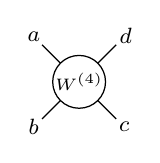
\begin{tikzpicture}[x=0.550cm, y=0.550cm, line width=0.450pt, baseline={([yshift=-0.6ex]0,0)}]
  \draw (0.000,0.000) -- (-0.431,0.431);
  \draw (0.000,0.000) -- (-0.431,-0.431);
  \draw (0.000,0.000) -- (0.431,-0.431);
  \draw (0.000,0.000) -- (0.431,0.431);
  \draw (-0.431,0.431) -- (-0.856,0.856);
  \draw (-0.431,-0.431) -- (-0.856,-0.856);
  \draw (0.431,-0.431) -- (0.856,-0.856);
  \draw (0.431,0.431) -- (0.856,0.856);
  \fill[white] (0.000,0.000) circle (0.610);
  \draw (0.000,0.000) circle (0.610);
  \node[font=\footnotesize, inner sep=0.6pt] at (0.000,0.000) {$\scriptstyle W^{(4)}$};
  \node[font=\footnotesize, inner sep=0pt, anchor=315] at (-0.919,0.919) {$a$};
  \node[font=\footnotesize, inner sep=0pt, anchor=45] at (-0.919,-0.919) {$b$};
  \node[font=\footnotesize, inner sep=0pt, anchor=135] at (0.919,-0.919) {$c$};
  \node[font=\footnotesize, inner sep=0pt, anchor=225] at (0.919,0.919) {$d$};
\end{tikzpicture}}
\diagramgap
\mbox{$\displaystyle +\,$\,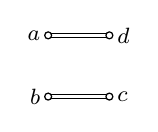
\begin{tikzpicture}[x=0.550cm, y=0.550cm, line width=0.450pt, baseline={([yshift=-0.6ex]0,0)}]
  \draw[double, double distance=0.837pt] (-0.707,0.707) -- (0.707,0.707);
  \draw[double, double distance=0.837pt] (-0.707,-0.707) -- (0.707,-0.707);
  \draw[fill=white] (-0.707,0.707) circle (0.080);
  \draw[fill=white] (-0.707,-0.707) circle (0.080);
  \draw[fill=white] (0.707,-0.707) circle (0.080);
  \draw[fill=white] (0.707,0.707) circle (0.080);
  \node[font=\footnotesize, inner sep=0pt, anchor=0] at (-0.877,0.707) {$a$};
  \node[font=\footnotesize, inner sep=0pt, anchor=0] at (-0.877,-0.707) {$b$};
  \node[font=\footnotesize, inner sep=0pt, anchor=180] at (0.877,-0.707) {$c$};
  \node[font=\footnotesize, inner sep=0pt, anchor=180] at (0.877,0.707) {$d$};
\end{tikzpicture}}
\diagramgap
\mbox{$\displaystyle +\,$\,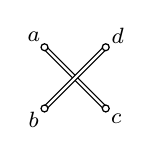
\begin{tikzpicture}[x=0.550cm, y=0.550cm, line width=0.450pt, baseline={([yshift=-0.6ex]0,0)}]
  \draw[double, double distance=0.837pt] (-0.707,0.707) -- (0.707,-0.707);
  \draw[double, double distance=0.837pt] (-0.707,-0.707) -- (0.707,0.707);
  \draw[fill=white] (-0.707,0.707) circle (0.080);
  \draw[fill=white] (-0.707,-0.707) circle (0.080);
  \draw[fill=white] (0.707,-0.707) circle (0.080);
  \draw[fill=white] (0.707,0.707) circle (0.080);
  \node[font=\footnotesize, inner sep=0pt, anchor=315] at (-0.827,0.827) {$a$};
  \node[font=\footnotesize, inner sep=0pt, anchor=45] at (-0.827,-0.827) {$b$};
  \node[font=\footnotesize, inner sep=0pt, anchor=135] at (0.827,-0.827) {$c$};
  \node[font=\footnotesize, inner sep=0pt, anchor=225] at (0.827,0.827) {$d$};
\end{tikzpicture}}
\diagramgap
\mbox{$\displaystyle +\,$\,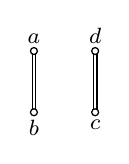
\begin{tikzpicture}[x=0.550cm, y=0.550cm, line width=0.450pt, baseline={([yshift=-0.6ex]0,0)}]
  \draw[double, double distance=0.837pt] (-0.707,0.707) -- (-0.707,-0.707);
  \draw[double, double distance=0.837pt] (0.707,-0.707) -- (0.707,0.707);
  \draw[fill=white] (-0.707,0.707) circle (0.080);
  \draw[fill=white] (-0.707,-0.707) circle (0.080);
  \draw[fill=white] (0.707,-0.707) circle (0.080);
  \draw[fill=white] (0.707,0.707) circle (0.080);
  \node[font=\footnotesize, inner sep=0pt, anchor=270] at (-0.707,0.877) {$a$};
  \node[font=\footnotesize, inner sep=0pt, anchor=90] at (-0.707,-0.877) {$b$};
  \node[font=\footnotesize, inner sep=0pt, anchor=90] at (0.707,-0.877) {$c$};
  \node[font=\footnotesize, inner sep=0pt, anchor=270] at (0.707,0.877) {$d$};
\end{tikzpicture}}
